The {\ttfamily oomph-\/lib} \char`\"{}architects\char`\"{} are (in no particular order)

 
\begin{DoxyImageNoCaption}
  \mbox{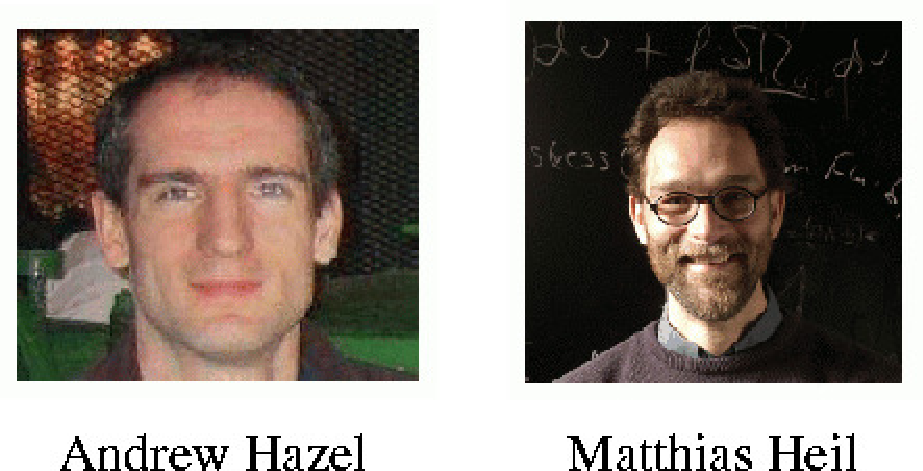
\includegraphics[width=0.75\textwidth]{architects}}
\end{DoxyImageNoCaption}


...assisted by former/current project/\+M\+Sc/\+PhD students and collaborators who made (or are still making) significant contributions to the development of the library (listed in reverse chronological order)\+:
\begin{DoxyItemize}
\item {\bfseries Thierry} {\bfseries Gonon} implemented the methodology to subtract singular (or non-\/singular) functions off solutions to the Poisson and Navier-\/\+Stokes equations.
\item {\bfseries Chris} {\bfseries Johnson} has provided many bug fixes.
\item {\bfseries Puneet} {\bfseries Matharu} works on the implementation of geometric multigrid solvers, particularly for Helmholtz equations.
\item {\bfseries Chihebeddine} {\bfseries Hammami} worked on the implementation of Yulii Shikhmurzaev\textquotesingle{}s interface formation theory.
\item {\bfseries Narjes} {\bfseries Akriche} worked on pseudo-\/resonances in acoustic fluid-\/structure interaction problems.
\item {\bfseries Aman} {\bfseries Rajvardhan} worked on implementing surfactant transport equations in two-\/ and three-\/dimensional geometries.
\item {\bfseries Jordan} {\bfseries Rosso} worked on topological fluid mechanics of the the Karman vortex street.
\item {\bfseries Florian} {\bfseries Molinier} did some early work on the coupled solution of the axisymmetric free-\/surface Navier-\/\+Stokes equations and the axisymmetric Foeppl von Karman equations.
\item {\bfseries Jonathan} {\bfseries Deakin} worked on a glaciology-\/related melt problem (and has since returned as PhD student to work on the numerical solution of acoustic fluid-\/structure interaction problems).
\item {\bfseries Draga} {\bfseries Pihler-\/\+Puzovic} worked on the the coupled solution of the Foeppl von Karman equations and the Reynolds lubrication equation to model wrinkling/fingering in elastic-\/walled Hele-\/\+Shaw cells.
\item {\bfseries Joris} {\bfseries Ferrand} worked on the solution of the Foeppl von Karman equations.
\item {\bfseries Harsh} {\bfseries Ranjan} worked on multiple solutions of Navier--Stokes flows in curved tubes.
\item {\bfseries Anton} {\bfseries Martinsson} implemented the machinery required to output {\ttfamily oomph-\/lib} data in paraview format, bypassing the need for running the time-\/consuming tecplot to paraview conversion scripts. He also implemented the displacement-\/based axisymmetric Foeppl von Karman equations.
\item {\bfseries Andr\'{e}} {\bfseries Von} {\bfseries Borries} is working on free-\/surface Navier--Stokes and lubrication theory problems.
\item {\bfseries Matthew} {\bfseries Walker} implemented P\+ML methods for the azimuthally Fourier-\/decomposed Helmholtz equations.
\item {\bfseries Joris} {\bfseries Ferrand} implemented the axisymmetric Foeppl von Karman equations.
\item {\bfseries Philippe} {\bfseries Mesnard} worked on acoustic F\+SI problems and introduced many improvements to {\ttfamily oomph-\/lib\textquotesingle{}s} machinery for handling such problems.
\item {\bfseries Florian} {\bfseries Molinier} worked on the coupling of the free surface Navier-\/\+Stokes equations and the axisymmetric Foeppl von Karman equations (in the context of simulating flows in elastic-\/walled Hele-\/\+Shaw problems).
\item {\bfseries David} {\bfseries Nigro} developed and implemented much of the machinery for acoustic fluid-\/structure interaction problems.
\item {\bfseries Matthew} {\bfseries Russell} implemented the Foeppl-\/von-\/\+Karman equations; he now continues to work on poro-\/elastic F\+SI problems.
\item {\bfseries Raphael} {\bfseries Perillat} worked on the simulation of flows in elastic-\/walled Hele-\/\+Shaw cells.
\item {\bfseries Robert} {\bfseries Harter} works on acoustic fluid-\/structure interaction problems.
\item {\bfseries Radu} {\bfseries Cimpeanu} implemented the P\+ML boundary conditions for the Helmholtz equations and the time-\/harmonic equations of linear elasticity.
\item {\bfseries Julio} {\bfseries Perez} {\bfseries Sansalvador} works on parallel unstructured mesh adaptation.
\item {\bfseries David} {\bfseries Shepherd} works on the numerical solution of micromagnetic problems.
\item {\bfseries Ray} {\bfseries White} is working on block preconditioners.
\item {\bfseries Nico} {\bfseries Bergemann} made (and continues to make) significant contributions to the adaptive unstructured mesh (re-\/)generation capabilities for free-\/surface problems.
\item {\bfseries Ben} {\bfseries Saxby} works on hp adaptivity and X\+F\+EM.
\item {\bfseries Michael} {\bfseries Crabb} worked on Discontinuous Galerkin (DG) methods.
\item {\bfseries Peter} {\bfseries Ashcroft} worked on eigenvalue problems.
\item {\bfseries Jeremy} {\bfseries van} {\bfseries Chu} contributed to the completion the tecplot to paraview conversion scripts and significantly extended the \href{../../paraview/html/index.html}{\tt the paraview tutorial.} He also developed the {\ttfamily Line\+Visualiser} machinery (which allows the extraction of computational data along lines in a higher-\/dimensional domain) and wrote the domain-\/based tube mesh.
\item {\bfseries Guilherme} {\bfseries Rocha} developed elements to simulate Hele-\/\+Shaw problems (by solving the free-\/surface Reynolds lubrication equations).
\item {\bfseries Ahmed} {\bfseries Wassfi} extended {\bfseries Tarak} {\bfseries Kharrat\textquotesingle{}s} work on the Helmholtz equation and implemented the Fourier-\/decomposed version of this equation.
\item {\bfseries Alexandre} {\bfseries Raczynski} keeps providing bug fixes and contributed to the completion the tecplot to paraview conversion scripts discussed in the \href{../../paraview/html/index.html}{\tt the paraview tutorial.}
\item {\bfseries David} {\bfseries Rutter} wrote the \href{../../linear_elasticity/periodic_load/html/index.html}{\tt tutorial for the linear elasticity equations.}
\item {\bfseries Tarak} {\bfseries Kharrat} implemented the Helmholtz elements and the methodology to apply the Sommerfeld radiation condition.
\item {\bfseries Luigi} {\bfseries Collucci} continued Benjamin Metz\textquotesingle{}s work and developed the interface from {\ttfamily oomph-\/lib} to {\ttfamily Triangle}.
\item {\bfseries Francisco} {\bfseries Jose} {\bfseries Blanco} {\bfseries Rodriguez} worked on free-\/surface problems and wrote the driver code that simulates the Rayleigh instability of an axisymmetric jet.
\item {\bfseries Wassamon} {\bfseries Phusakulkajorn} worked on C1-\/continuous triangular finite elements for shell, beam and biharmonic problems.
\item {\bfseries Benjamin} {\bfseries Metz} worked on adaptivity and solution transfer for unstructured meshes.
\item {\bfseries Amine} {\bfseries Massit} worked on outflow boundary conditions for Navier-\/\+Stokes problems and physiological F\+SI problems based on meshes generated by \href{http://www.vmtk.org/}{\tt vmtk}.
\item {\bfseries Patrick} {\bfseries Hurley} works on free surface Navier-\/\+Stokes problems.
\item {\bfseries Andy Gait} worked on parallelisation, in particular the problem distribution and the subsequent distributed mesh adaptation.
\item {\bfseries Angelo Simone} wrote python scripts that convert {\ttfamily oomph-\/lib\textquotesingle{}s} output to the vtu format that can be read by \href{http://www.paraview.org}{\tt paraview}; see \href{../../paraview/html/index.html}{\tt the paraview tutorial} for details.
\item {\bfseries Sophie} {\bfseries Kershaw} worked on the Navier-\/\+Stokes equations in spherical coordinates.
\item {\bfseries Floraine} {\bfseries Cordier} developed the driver codes and tutorials for the \href{../../interaction/fsi_channel_with_leaflet/html/index.html}{\tt flow past the elastic leaflet} and \href{../../interaction/turek_flag/html/index.html}{\tt Turek \& Hron\textquotesingle{}s F\+SI benchmark}. In the process she significantly extended {\ttfamily oomph-\/lib\textquotesingle{}s} F\+SI capabilities.
\item {\bfseries  Stefan Kollmannsberger} and his students Iason Papaioannou and Orkun Oezkan Doenmez developed early versions of the code for \href{../../interaction/turek_flag/html/index.html}{\tt Turek \& Hron\textquotesingle{}s F\+SI benchmark} and its \href{../../navier_stokes/turek_flag_non_fsi/html/index.html}{\tt non-\/\+F\+SI counterpart.}
\item {\bfseries Cedric Ody} developed the {\ttfamily Young\+Laplace} elements and their refineable counterparts to study capillary statics problems.
\item {\bfseries Alice} {\bfseries Gaertig} developed interfaces to the third-\/party mesh generators \href{http://www.cs.cmu.edu/~quake/triangle.html}{\tt {\ttfamily Triangle}, } \href{http://wias-berlin.de/software/tetgen//}{\tt {\ttfamily Tet\+Gen}, }, \href{http://members.shaw.ca/bjoe/}{\tt {\ttfamily Geompack++}, } and \href{http://www.dimap.ufrn.br/~mfsiqueira/Marcelo_Siqueiras_Web_Spot/cqmesh.html}{\tt {\ttfamily C\+Q\+Mesh}. }
\item {\bfseries Claire} {\bfseries Blancon} developed the demo drivers for the collapsible channel problem (with and without fluid-\/structure interaction).
\item {\bfseries Nick} {\bfseries Chapman} worked on the implementation of triangular and tet-\/elements.
\item {\bfseries Chris} {\bfseries Gold} implemented explicit timestepping schemes.
\item {\bfseries Phil} {\bfseries Haines} worked on bifurcation detection and tracking for the Navier-\/\+Stokes equations and developed the formulation of the equations in plane polar coordinates.
\item {\bfseries Richard} {\bfseries Muddle} worked on the block preconditioning techniques for the biharmonic (and many other) equations, and parallel solvers.
\item {\bfseries Glyn} {\bfseries Rees} worked on iterative linear solvers and multigrid
\item {\bfseries Alberto} {\bfseries de} {\bfseries Lozar} worked on 3D free-\/surface Navier-\/\+Stokes problems.
\item {\bfseries Jonathan} {\bfseries Boyle} developed the initial interfaces to third-\/party iterative solvers and is now involved in the further parallelisation of the code and the implementation and application of block-\/preconditioning techniques for Navier-\/\+Stokes and fluid-\/structure interaction problems.
\item {\bfseries Renaud} {\bfseries Schleck} completed the octree-\/based mesh refinement procedures and wrote the M\+P\+I-\/based parallel assembly routines and the interfaces to Super\+L\+U\+\_\+dist.
\item {\bfseries Sharaf} {\bfseries Al-\/\+Sharif} provided the initial implementation of nodal spectral elements.
\item {\bfseries Daniel} {\bfseries Meyer} used oomph-\/lib to study a variety of axisymmetric Navier-\/\+Stokes problems, with and without free surfaces, and developed drafts for many of our tutorials.
\item {\bfseries Alexandre} {\bfseries Klimowicz} worked on block-\/preconditioning methods.
\item {\bfseries Jean-\/\+Michel} {\bfseries Lenoir} implemented the first part of the octree-\/based 3D mesh refinement procedures.
\item {\bfseries Gemma} {\bfseries Barson} provided the initial implementation for the 2D Delaunay mesh generation procedures.
\end{DoxyItemize}

We\textquotesingle{}re always looking for more help! Get in touch if you\textquotesingle{}re interested in joining the team.



 

 \hypertarget{index_pdf}{}\section{P\+D\+F file}\label{index_pdf}
A \href{../latex/refman.pdf}{\tt pdf version} of this document is available. \end{document}
